\chapter{Resilience analysis}
% - 0. basic hysteresis/irreversibly result 1. Pumps wealth out on way up and way down 2. class 3. map regimes


\begin{figure}
\centering
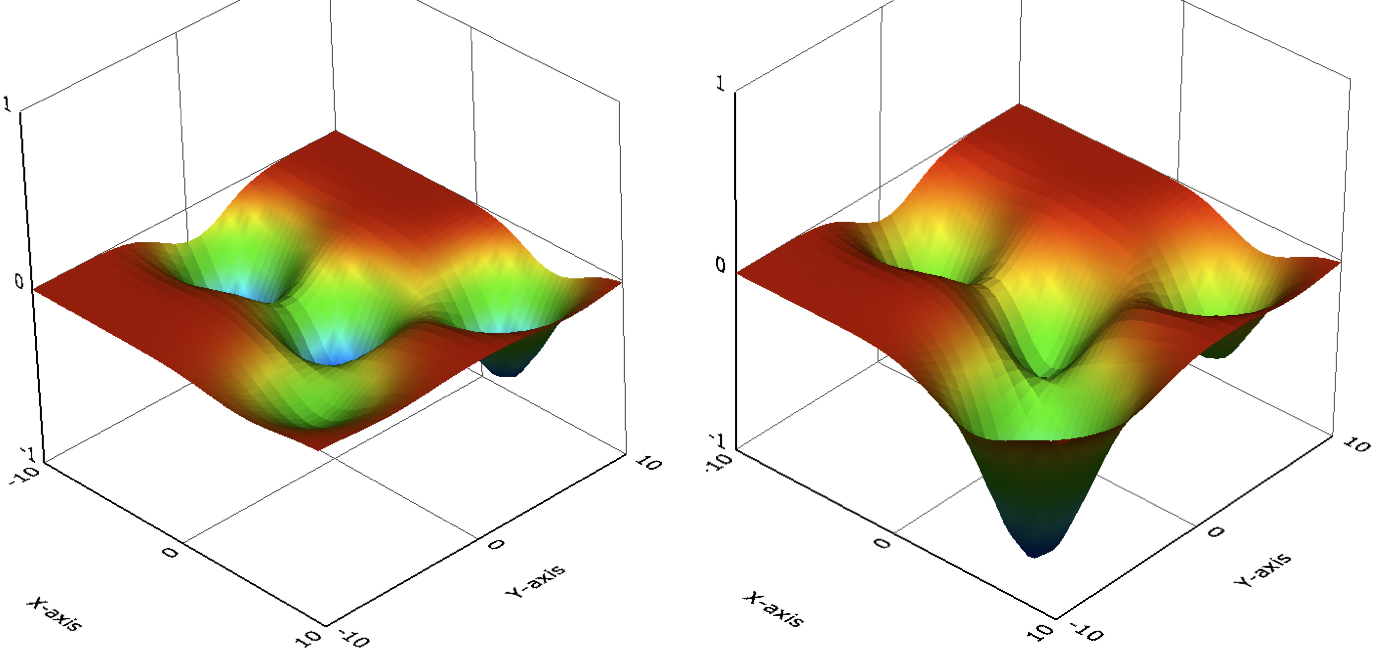
\includegraphics{fig/basins.png}
\caption{Basins of attraction}
\label{fig-basins}
\end{figure}

Historically low interest rates, and financial crises, have been a primary driver of rapid inflows of financial capital, accelerating the process, which raises the question of what will happen as interest rates rise. The analysis suggests however that there is hysteresis, that both the economic upswing and the downswing pull wealth out of communities, like a kind of ratchet or peristaltic pump. We analyze and model these dynamics in the resilience Chapter, %Chapter~\ref{chapter-resilience}

The model gives a resilience result which is that shared wealth through housing is not resilience.

It can also be used with a driven version of the model to show that the model pumps wealth out on the upswing and on the downswing - like a kind if ratchet.


Once we have this model it is useful for also understanding the wealth effects, in particular the resilience dynamics
Resilience is an under used concept in economic analysis for a few reasons. We show an example of that type of analysis based on hysteresis here. 


There are two types of resilience questions when any system is shocked, does it return to an equilibrium state, the stability question, and does it return to the same kind of equilibrium---the hysteresis question. % We focus on the latter question.  

\section{Definitions of resilience}

The concept of resilience has been used to understand the persistence and vulerabilty of high dimensioanl social and ecological systems %\cite{several reviews}
but is usually defined either verbally or formally in terms of low dimensional dynamical systems. Recent work has begun to look at how to extend it to higher dimensional systems \cite{gao_universal_2016}. 

Litturature on resilience is part of a larger body of work on several distinct stability concepts. 
Grimm and Wissel reviewed stability terms from the ecological literature \cite{grimm_what_2011, grimm_babel_1997} and identified three core underlying concepts \footnote{They reviewed 163 definitions and 70 distinct terms.}. The first was \textbf{constancy}, the degree to which the some element of a system resists perturbation. The second was engineering resilience, the ability of a system to \textbf{bounce back} from a disturbance.  The third was the \textbf{viability of some feature of a system in the long term}. % Did the property actually die out or did it last?

The concept of resilience from the ecological literature is related to this this final stability concept. Holling originally defined resilience as determining ``the \textbf{persistence of relationships within a system}.'' It is, he continues, ``a measure of the ability of these systems to absorb changes of state variables, driving variables, and parameters, and still persist” \cite{holling_resilience_1973}. %(Holling 1973, p. 17 - checked page and quote DONE) %In this definition resilience is the property of the system and persistence or probability of extinction is the result.


% Ludwig, Jones and Holling, Qualitative analysis of insect out- break systems: the spruce budworm and forest , Journal of Ani- mal Ecology (1978), 47 , 315-332.2. Polking, Boggess and Arnold, Differential Equations , 158-161. October 6, 1977 issue of Nature Magazine (Vol. 269, pg. 471)

His definition was developed in the context of this formal modelling but was itself verbal and qualitative. More recently Walker et al. define resilience as %``Resilience is 
``the \textbf{capacity of a system to absorb disturbance and reorganize while undergoing change so as to still retain essentially the same function, structure, identity, and feedbacks}'' \cite{walker_resilience_2004}.
 % Resilience is the capacity of systems to maintain their identity, feedbacks, structure, and pattern of functioning as they pass through transformations. 
Empirically, Marten Scheffer and others look at %who developed a toolkit for measuring advance indicators of critical transitions, define 
measure resilience using the ``\textbf{magnitude of disturbance a system can tolerate before it shifts into a different state}'' \cite{scheffer_critical_2009}.
% (Critical Transitions in Nature and Society, Dakos critical transitions advance warning toolkit website glossary has this as the definition of resilience)



Work on networks and resilience defines resilience as ``a system’s \textbf{ability to adjust its activity to retain its basic functionality} when errors, failures and environmental changes occur'' \cite{gao_universal_2016}. %(Gao et al. 2016). 
They say this has traditionally been defined for ``low-dimensional models with a few interacting components'' in the following way:
% For the low dimensional defintion, they cite Sole, R. V. & Montoya, M. Complexity and fragility in ecological networks. Proc. R. Soc. Lond. B 268, 2039–2045 (2001) ** 

\begin{equation}
   \frac{dx}{dt} = f(\beta, x)
\end{equation}
Where $f(\beta, x)$ is the system's dynamics, $\beta$ is changing environmental conditions, and the system has several stable fixed points or regimes. The system begins near at one of the fixed points and is initially stable.

\begin{equation}
   f(\beta, x_0) = 0
\end{equation}

\begin{equation}
   \frac{\partial f}{\partial x} \bigg|_{x = x_0} < 0
\end{equation}
Over changes in the tunable parameter $\beta$, the system can reach a biffurcaiton or become non-analytic, and transition to an alternative stable state or regime.

Neubert and Caswell describe a range of measures for how ecological systems respond to perturbations \cite{neubert_alternatives_1997}. These include the
rate at which perturbations decay, % to stable equilibrium decay, most often based on the eigenvalues at equilibrium, which gives rate of recovery asymtotically as time goes to infinity, and % (copied note. check this is paraprhased properly) %New measures of transient response
reactivity, and the maximum possible growth rate immediately after perturbation.
%'These indices measure the extent and duration of transient growth in models with asymptotically stable equilibria. They are: 

%\begin{enumerate}
%   \item \textbf{reactivity} (the maximum possible growth rate immediately following the perturbation), the 
%   \item \textbf{maximum amplification} (the largest proportional deviation that can be produced by any perturbation), and the 
%   \item \textbf{time at which this amplification occurs}. 
%\end{enumerate}


%------------------------------------------------------------------


% [1] J. Gao, B. Barzel, and A.-L. Barab ́asi, “Universal resilience patterns in complex net- works,” Nature, vol. 530, no. 7590, pp. 307–312, 2016.
% [2] V. Grimm and J. M. Calabrese, “What is resilience? A short introduction,” in Viability and Resilience of Complex Systems, ser. Understanding Complex Systems, G. Deffuant and N. Gilbert, Eds. Berlin: Springer, 2011, pp. 3–13.
% [3] V. Grimm and C. Wissel, “Babel, or the ecological stability discussions: An inventory and analysis of terminology and a guide for avoiding confusion,” Oecologia, vol. 109, no. 3, pp. 323–334, 1997.
% [4] C. Holling, “Resilience and stability of ecological systems,” Annual Review of Ecology and Systematics, vol. 4, pp. 1–23, 1973.
% [5] B. Walker, C. S. Holling, S. Carpenter, and A. Kinzig, “Resilience, adaptability and transformability in social-ecological systems,” Ecology and Society, vol. 9, no. 2, 2004.
% [6] M. Scheffer, Critical Transitions in Nature and Society, Princeton, 2009.
% [7] M. G. Neubert and H. Caswell, “Alternatives to resilience for measuring the responses
% of ecological systems to perturbations,” Ecology, vol. 78, no. 3, pp. 653–665, 1997.

\subsection{Endogenous cycling}
Paul suggests that resilience is usually studied in the context of a system which endogenously shifts between two alternative regimes.

This is false, in the vast majority of cases resilience in ecological systems is studied in the context of a system which 

That being said, endogenous cycling is caused by a feedback cycle which causes the system to cycle between distinct high and low employment regime within a single region of the state space.

There is also a region near the boundaries, kicks to state through endogenous randomness can also cause the system to cross the boundary from one region to another.


\section{Resilience background}

This section explores the resilience dynamics of distribution of wealth within a class of market models.  

Using a systems design approach and looking at resilience measures and alternative regimes gives insights into patterns of distribution and how that shapes wealth. 

The two significant concepts of resilience for this work are the relationship between distinct alternative regimes and patterns of cycling within a single regime. 

\section{What is resilience and how is it connected to this work}

Resilience is a concept that has to with the way in which a system resists disturbance or maintains identity through disturbance. The concept has emerged independently with different, but related definitions in various fields. 
There are a class of systems that this idea of resilience should be applicable or illuminating for, however the concepts and measures that exist already are ill-suited to the dynamics of the system. 
The work in this thesis draws from the measures from existing measures and concepts of resilience from various discipline to evolve a measure that can apply to this other class of systems. 

Shaping this core broadly applicable concept that 
We can approach change in various systems using technical tools that are transferable. 
The concept 

\section{Resilience in engineering}

In engineering, Resilience is defined as the return properties of a system. 
It is the measures relating to how a system comes back to its stable equilibrium or stable state. For example if you push a branch on a tree, it will oscillate and settle back to its resting position. 

Stability properties are important in engineering because engineers are responsible for signing off the performance of system, whether the the system is a bridge or a chemical reactant or an electrical circuit. Stability is an aspect of the system's behaviour. The engineer needs measures to predict the stability of the system when it's perturbed. (Specific) 

Engineering resilience is distinct from the failure zones or the threshold of failure - for example the level of force/weight or number of stress cycles that would be required to collapse a bridge. While those measures pertain the thresholds beyond which the system would fail, resilience is about describing how the system recovers from perturbations that do not break it. 

The primary measure is how long the system takes to return to its equilibrium, i.e. the return time. (Equation) There are seven measures, listed in table XYZ that pertain to return to equilibrium properties.  (Table)

There is some variation in the use of the concept in specific disciplines of Engineering. For example, in transport engineering it has something to do with traffic flow.

\section{Resilience in ecology}

In Ecology resilience is defined as the way in which systems maintain identity through transformations. 

In engineering, the concept of resilience centres on the idea of a single equilibrium. If the system is not disturbed, it will stay at equilibrium and the resilience measures account for the system's return to this equilibrium. In the ecology, on the other hand, instead of a single equilibrium the underlying pattern of the system has a dynamic structure. For example the ecosystem of a forest contains ongoing cycles of life and death and evolving patterns and interactions and yet sustains its identity as a forest. 

An ecosystem can experience big shocks or disturbances without losing its basic identity. For example, there can be drought, floods, fire, species loss, etc and the forest can recover and continue to be a forest. (The forest can regrow, one species might replace another and the forest changes but it doesn't necessarily stop being a forest.) But some disturbances can tip the ecosystem over into a different pattern of functioning. For example if the land is cleared and animals come into to graze the seedling trees so that they do not grow back, the forest can transition to a grassland ecosystem. Or if the region becomes dry enough, the forest can transition to become a desert. 

In ecology these alternative patterns of a system that may be identified as a forest, grassland, or desert are called regimes. In Ecological resilience studies, this concept of regimes replaces the simpler idea of equilibrium, differing both because the underlying pattern is more complex and because there are multiple regimes that the ecosystem of the same land can shift between. 

Part of what resilience in ecology is getting at, then, is what kind and how big the disruption can be before the ecosystem becomes a different kind of ecosystem. Resilience measures describe the properties of these distinct regimes and the relations between them. The most common measure is the size of the perturbation the system can withstand without transitioning into an alternative pattern of functioning or regime.  

This approach to resilience was introduced by C.S. Holling with his 1973 paper on a Spruce Budworm model of a forest ecosystem. In this paper he argued that there was an evolving interrelationship/feedback cycle between Spruce growth/regrowth and the population of Spruce Budworms that eat them. This interaction drove ongoing cycles of forest recovery and collapse. 

Holling's work established the concept of these kinds of cycled and alternative regimes in ecosystems. Subsequent work by Marten Scheffer in lake eutrophication validated that alternative regimes appear in ecosystems in the real world. Now there is a database tracking thresholds and regime shifts in ecological systems with over a hundred entries showing its common.  ([https://www.resalliance.org/thresholds-db](https://www.resalliance.org/thresholds-db)) 

In ecology, this idea of resilience has evolved into a dynamic concept that is important in climate change science and ecological conservation. Resilience measures show how a system maintains identity through change by measuring the relationship between regimes, that is how close a system is to transitioning to a different regime or pattern of functioning. Thus the concept of ecological resilience and alternate regimes give tools to understand what is possible for an ecosystem. This give insight both into how ecosystems can be preserved but also what happens when they transform. 




\section{Resilience in social systems}

The ecological concept of Resilience has since been applied widely to various systems across disciplines (*INSERT EXAMPLES*). Frances Westley applies Holling's idea of alternative regimes to social systems as the basis for a theory of social innovation. 

Westley defines social innovation as ``a change in the routines, resource flows, authority flows or beliefs in any social system.'' According to Westley ``a successful social innovation also has durability and broad impact.'' 
Her studies in social innovation focus on how individuals, groups, or institutions are able to shift social systems to achieve certain goals. 

Westley's research question is how social systems transform. This frame differs from the majority of resilience work in engineering and ecology because the focus there tends to be on maintaining the integrity of the system, whereas Westley's work is focused on how to move between regimes. 

For example, in the Great Bear Rainforest in British Columbia in the late 1990's (??) clearcutting for pulp and paper was threatening some of the last old old growth forests in the region and disrupting the lives of people who depended on them. Over years of unchecked logging combined with a history of land appropriation, there was ongoing local resistance. In 199X images of the devastation spread through international media and led to a boycott of paper products from clearcutting. This moment of crisis brought the forestry industry to the table. After a carefully structured process of conversation and engagement between community organizers, political leaders, and industry they put the Great Bear Rainforest under Indigenous community control. 

This change in governance structure can be understood social system that can be understood as a regime change because there were a set of patterns and feedbacks holding the old system in place and and there new set of patterns and feedbacks holding the new system in place. Each regime has a distinct pattern of functioning or identity. 

The idea of resilience in social innovation illuminates how the patterns of different regimes structure the social systems. What is different about the two regime in the case of the Great Bear Rainforest is the distribution of the flow of money and power - or the the language of social innovation, resources and authority. This changed the routines and habits of the people making up the social system as they became more directly involved in managing the forest. The result is that the ancient Great Bear Rainforest survived. 

The study of resilience within social innovation looks at how actors within  systems play a role in shaping transformation of interconnected social-ecological systems. Westley specifically studies individuals, groups, or institutions who have the intention to shift social systems to achieve certain goals. This means that there is a directed strategic nature to the agents. This is illustrated by the case of the Great Bear Rainforest by the different stakeholders from industry, community and governance who are are all actively working to achieve specific goals. However none of these actors are outside outside the system. Even those with power cannot completely control the system. Their efforts interact with the actions of others and the broader context of the whole

Social systems are dynamic. There is no fixed equilibrium and yet they have clusters of properties that persist and can prove difficult to change. These patterns with distinct identities are described in social innovation theory as regimes. These patterns can pertain to various feature, from the routines that structure interactions to resource flows within the system. In the example of the Great Bear Rainforest, under the previous system the resources and money flowed out of the community and decisions were made by distant corporations. The shift in governance structurally affected both the ecosystem and the culture of the communities. When they shifted to community governance, the emphasis shifted away from extraction and toward investing and building the forest and the community. (ADD CONCRETE DETAILS/NUMBERS?) 

Sometimes people can achieve their goals and sometimes they do not and it depend on both what they do and the state of the system. In her grounded theory work studying people who have attempted and succeeded in changing systems, Westley observed that sometimes there are moments of opportunity that make shifts in the system possible.  In the rainforest example, there were years of Indigenous organizing and building an environmental movement. 
The change became possible at a particular moment when commodity prices were placing pressure on the industry and coordination between local and national environmentalists resulting in international boycotts of pulp and paper products from clearcut forest, particularly across Europe. The indigenous organizers were able to achieve more in this moment of opportunity.

According to Westley a successful social innovation also ``has durability and broad impact.'' This is a description of the change but it also illuminates how the resilience concept of regimes is useful. One feature of systems is that a set of feedback loops will hold patterns of interactions, resources flows, etc in place. Many changes simply die out.  The changes that last do so because they change the flows and dynamics in ways that are held in place by new feedback loops.  Social Innovation theorists have used the concept of regimes to explain this phenomena. If the system state is perturbed enough another set of patterns can come to dominate.  (MAKE SURE THESE TERMS ALIGN WITH THE PRECISE TERMINOLOGY USED LATER) In the example, after the shift to the community governance that became self-reinforcing as different feedback loops emerged to structure the building of relationships and institutional structures, community habits, networks of support, and resource flows. 

\section{Role of this thesis}

What has been articulated in Social innovation theory is a story of how feedback loops hold the patterns in place  and how systems can switch between sets of patterns. Westley and others have applied the concept of resilience as an explanatory framework, rather than as a a precise mathematical statement. 
The thesis seeks to operationalize these concepts within a formal model in the context of social systems. 


- By operationalizing into this model, we can patterns in how systems shift between regimes. Specifically in this thesis the models show where in the systems there are opportunities - ie the system is more vulnerable or -open to change. 
- In practice regimes change can move you into a more or less desired state. Here I focus on opportunities and interventions. 
- Inventions are \dots
- By looking at where the system has opportunity to change this work illuminates how actors might be able to identify opportunities for regime change. 
- 




prosperity and resilience/vulnerability/opportunity in the context of many agents.











he analysis has been applied conceptually, rather than as a precise mathematical statement. Thus far, in the study of social innovation 

Routines, resource authority flow and beliefs. 

International concern
Boycotts 
Political movement

Effective local movement established an indigenously led sustainable forest and tenure
It 



Community leaders were able to establish a 




Social innovation involves interventions or actions 




She studies I

Change in technology and demand for wood. 

For example, she looks at how various countries responded to the AIDS crisis and how activists in certain shaped 

There's a debate about how systems transform. 
Impersonal forces of history like the development of agriculture
She's studying the phenomena of change in order to inform 
The research is about how people try to change the word. 

(ie. a system consisting of different interconnected entities such as  individuals, groups, and institutions relating to each other and forming a whole.)

An interdependence of a social and cultural element 

Series of interrelationships between individuals and groups and institutions forming a whole. 



% [[adaptive cycle]]




Recreate their images in low resolution (\textbf{phase diagram, example trajectories, policy performance}).

Alternative experiment ideas include:

\begin{enumerate}
\item Find and trace the boundary by brute force. They currently use mean field approximations or \textbf{brute force simulations} to identify the phases, barriers and regimes/patterns in phase diagrams of the economy (add detail).
\item Find and trace the boundary by ab initio methods. Try ab initio methods from chemistry to find and \textbf{trace the boundary}. Identify a generic regime boundary. Identify latent alternative states.
   \item \textbf{Characterize the boundary}. Characterize save/dangers near regime boundaries.
   \item Systematically \textbf{vary the model} in the direction likely to change the set of patterns of behaviours. \textbf{Identify new phases}, patterns without knowing them in advance../new regimes.
   \item Systematically explore/intelligently explore a space of alternative \textbf{interventions}.. — select hyper-parameters/model the parameter space. Model/think about the geometry of the intervention space/and the dimension of it.. — ways to control what levers.. in time, space, etc..? VERY LARGE SEARCH SPACE ETC..
   \item Characterize/link with the \textbf{adaptive cycle} — connectivity wealth, etc..
Adaptive cycle currently treated as metaphorical .. measure the predicted effect in these models and compare with data.. capital etc..
\item Look at \textbf{traps}, and interventions using an energy \textbf{barrier framework}.
Phenomena including the \textbf{Paradox of thrift, Liquidity traps.}
\item \textbf{Network efficiency} and others under different classes of attacks? measure of economic efficiency with frictions, capital, trust etc.. recovery times. e.g. Trust collapse network sizes.
\item \textbf{Math of paradigm shift in stylized model} - openings through cycling. resilience and the adaptive cycle — a cycle that allows for adaptation.. FILL IN DETAILS.


\item Look at the effect of money on the shape of endogenous crises
\item Look at the effect of advance/pre triggering of endogenous crises
\item Look at methods to reduce/change the depth of crises/peaks
\item Compare one large intervention with continuous intervention and lots of small interventions, look at timing effects.

\item The high-throughput highway to computational materials allows comparison of a whole class of models and policy inventions..

\item The way to study this is to study 1. model changes 2. policy changes (geometry of the system). 
\end{enumerate}





\section{How to compare multiple replicate runs?}

Compare with standard deviation (CV is a dimensionless form of this)

You could look at the\textbf{ Standard deviation} (SD) or \textbf{Standard Error of the Mean} (SEM) which will give you an idea of how close the replicate values are to each other.  


``The standard error of the mean (SE of the mean) \textbf{estimates the variability between sample means that you would obtain if you took multiple samples} from the same population. The standard error of the mean estimates the variability between samples whereas the standard deviation measures the variability within a single sample.''

best way to calculate the variability between assays and duplicates/triplicates is \textbf{CV=(SD/mean)*100}. The lower CV the better, It should be less than 20\%. 
I think some people use <15 percent CV as a valid result, if it is higher than 15\%, then you shouldn't consider that duplicate/triplicate.

``In order to express the precision, or repeatability, of immunoassay test results, rresearchers in the social and  behavioral sciences typically report two measures of the \textbf{Coefficient of Variability}  (CV) in their publications:  the  Inter - Assay CV and the Intra - Assay CV.  The CV is a dimensionless number defined as the \textbf{standard deviation of a  set of measurements divided by the mean of the set}. ``

`` The degree to which the duplicate results differ 
can be expressed by calculating t
he standard deviation of the two results and converting it to the CV. ``
\cite{https://www.salimetrics.com/assets/documents/Spit_Tips_-_Inter__Intra_Assay_Coefficients_of_Variability.pdf}


``If \textbf{absolute values are similar, populations can be compared using their standard deviations}. But if they differ markedly (for example, the weights of mice and elephants), or are of different variables (for example, weight and height), then you need to use a standardized measure - such as the coefficient of variation. The coefficient of variation (CV) for a sample is the standard deviation of the observations divided by the mean. The most common use of the coefficient of variation is to assess the precision of a technique. It is also used ass a measure of variability when the standard deviation is proportional to the mean, and as a means to compare variability of measurements made in different units.''
\cite {https://www.researchgate.net/post/How_to_calculate_the_inter_assay_and_intra_assay_vatiations }



\subsection{What are replicat runs vs repeats}
(assume the system is stationary?)

'Replicates are multiple experimental runs with the same factor settings.' 'Repeat and replicate measurements are both multiple response measurements taken at the same combination of factor settings; but repeat measurements are taken during the same experimental run or consecutive runs, while replicate measurements are taken during identical but different experimental runs, which are often randomized.'
\cite{http://support.minitab.com/en-us/minitab/17/topic-library/modeling-statistics/doe/basics/replicates-and-repeats-in-designed-experiments/}
``Replicates are duplicate runs of the entire experiment.
The latter is preferable for minimising errors. Sample size calculations apply to replicates not repeats.''

I need to actually calculate the CV for each sample: \cite{http://r.789695.n4.nabble.com/Need-to-calculate-within-and-between-run-CV-td866024.html}
  - within run (between replicates) - that's easy to do in Excel
  - between run - that's the problem.
  aov' or 'lme'? 
